%Version 3 December 2023
% See section 11 of the User Manual for version history
%
%%%%%%%%%%%%%%%%%%%%%%%%%%%%%%%%%%%%%%%%%%%%%%%%%%%%%%%%%%%%%%%%%%%%%%
%%                                                                 %%
%% Please do not use \input{...} to include other tex files.       %%
%% Submit your LaTeX manuscript as one .tex document.              %%
%%                                                                 %%
%% All additional figures and files should be attached             %%
%% separately and not embedded in the \TeX\ document itself.       %%
%%                                                                 %%
%%%%%%%%%%%%%%%%%%%%%%%%%%%%%%%%%%%%%%%%%%%%%%%%%%%%%%%%%%%%%%%%%%%%%

%%\documentclass[referee,sn-basic]{sn-jnl}% referee option is meant for double line spacing

%%=======================================================%%
%% to print line numbers in the margin use lineno option %%
%%=======================================================%%

%%\documentclass[lineno,sn-basic]{sn-jnl}% Basic Springer Nature Reference Style/Chemistry Reference Style

%%======================================================%%
%% to compile with pdflatex/xelatex use pdflatex option %%
%%======================================================%%

%%\documentclass[pdflatex,sn-basic]{sn-jnl}% Basic Springer Nature Reference Style/Chemistry Reference Style


%%Note: the following reference styles support Namedate and Numbered referencing. By default the style follows the most common style. To switch between the options you can add or remove “Numbered” in the optional parenthesis. 
%%The option is available for: sn-basic.bst, sn-vancouver.bst, sn-chicago.bst%  
 
%%\documentclass[pdflatex,sn-nature]{sn-jnl}% Style for submissions to Nature Portfolio journals
%%\documentclass[pdflatex,sn-basic]{sn-jnl}% Basic Springer Nature Reference Style/Chemistry Reference Style
\documentclass[pdflatex,sn-mathphys-num]{sn-jnl}% Math and Physical Sciences Numbered Reference Style 
%%\documentclass[pdflatex,sn-mathphys-ay]{sn-jnl}% Math and Physical Sciences Author Year Reference Style
%%\documentclass[pdflatex,sn-aps]{sn-jnl}% American Physical Society (APS) Reference Style
%%\documentclass[pdflatex,sn-vancouver,Numbered]{sn-jnl}% Vancouver Reference Style
%%\documentclass[pdflatex,sn-apa]{sn-jnl}% APA Reference Style 
%%\documentclass[pdflatex,sn-chicago]{sn-jnl}% Chicago-based Humanities Reference Style

%%%% Standard Packages
%%<additional latex packages if required can be included here>

\usepackage{graphicx}%
\usepackage{multirow}%
\usepackage{amsmath,amssymb,amsfonts}%
\usepackage{amsthm}%
\usepackage{mathrsfs}%
\usepackage[title]{appendix}%
\usepackage{xcolor}%
\usepackage{textcomp}%
\usepackage{manyfoot}%
\usepackage{booktabs}%
\usepackage{algorithm}%
\usepackage{algorithmicx}%
\usepackage{algpseudocode}%
\usepackage{listings}%
\usepackage{underscore}
\usepackage{float}
\usepackage{tabularx}
\usepackage{booktabs}
\usepackage{hyperref}
\usepackage{siunitx}
\usepackage{pgfplotstable}
\usepackage{booktabs}
\usepackage{array}
\usepackage{colortbl}
\usepackage{tcolorbox}
\usepackage{amsmath}
\usepackage{multirow}
\usepackage{soul,color}
\usepackage[utf8]{inputenc}
\usepackage{glossaries}

\makeglossaries
\newacronym[plural={LLMs}]{llm}{LLM}{Large Language Model}
\newacronym{nlp}{NLP}{Natural Language Processing}
\newacronym{svm}{SVM}{Support Vector Machine}
\newacronym{mlp}{MLP}{Multilayer Perceptron}
\newacronym{xgb}{XGBoost}{eXtreme Gradient Boosting}
\newacronym{bert}{BERT}{Bidirectional Encoder Representations from Transformers}
\newacronym{llama}{Llama}{Large Language Model Meta AI}



\soulregister\cite7
\soulregister\ref7
\soulregister\pageref7
 \pgfplotsset{compat=1.18}
%%%%

%%%%%=============================================================================%%%%
%%%%  Remarks: This template is provided to aid authors with the preparation
%%%%  of original research articles intended for submission to journals published 
%%%%  by Springer Nature. The guidance has been prepared in partnership with 
%%%%  production teams to conform to Springer Nature technical requirements. 
%%%%  Editorial and presentation requirements differ among journal portfolios and 
%%%%  research disciplines. You may find sections in this template are irrelevant 
%%%%  to your work and are empowered to omit any such section if allowed by the 
%%%%  journal you intend to submit to. The submission guidelines and policies 
%%%%  of the journal take precedence. A detailed User Manual is available in the 
%%%%  template package for technical guidance.
%%%%%=============================================================================%%%%

%% as per the requirement new theorem styles can be included as shown below
% \theoremstyle{thmstyleone}%
% \newtheorem{theorem}{Theorem}%  meant for continuous numbers
%%\newtheorem{theorem}{Theorem}[section]% meant for sectionwise numbers
%% optional argument [theorem] produces theorem numbering sequence instead of independent numbers for Proposition
% \newtheorem{proposition}[theorem]{Proposition}% 
%%\newtheorem{proposition}{Proposition}% to get separate numbers for theorem and proposition etc.

% \theoremstyle{thmstyletwo}%
% \newtheorem{example}{Example}%
% \newtheorem{remark}{Remark}%

% \theoremstyle{thmstylethree}%
% \newtheorem{definition}{Definition}%

\raggedbottom
%%\unnumbered% uncomment this for unnumbered level heads

\begin{document}

\title[Article Title]{Predicting retracted research}

%%=============================================================%%
%% GivenName	-> \fnm{Joergen W.}
%% Particle	-> \spfx{van der} -> surname prefix
%% FamilyName	-> \sur{Ploeg}
%% Suffix	-> \sfx{IV}
%% \author*[1,2]{\fnm{Joergen W.} \spfx{van der} \sur{Ploeg} 
%%  \sfx{IV}}\email{iauthor@gmail.com}
%%=============================================================%%

\author[*]{\fnm{Aaron HA} \sur{Fletcher}}
\email{ahafletcher1@sheffield.ac.uk}
% \equalcont{These authors contributed equally to this work.}
\author[*]{\fnm{Mark} \sur{Stevenson}}
\email{mark.stevenson@sheffield.ac.uk}
% \equalcont{These authors contributed equally to this work.}

% \author[1,2]{\fnm{Third} \sur{Author}}\email{iiiauthor@gmail.com}
% \equalcont{These authors contributed equally to this work.}

\affil[*]{\orgdiv{School of Computer Science}, \orgname{The University of Sheffield}, \orgaddress{\street{Regent Court}, \city{Sheffield}, \postcode{S1 4DP},  \country{United Kingdom}}}

% \affil[2]{\orgdiv{Department}, \orgname{Organization}, \orgaddress{\street{Street}, \city{City}, \postcode{10587}, \state{State}, \country{Country}}}

% \affil[3]{\orgdiv{Department}, \orgname{Organization}, \orgaddress{\street{Street}, \city{City}, \postcode{610101}, \state{State}, \country{Country}}}

%%==================================%%
%% Sample for unstructured abstract %%
%%==================================%%

\abstract{

\textbf{Background:} Retractions undermine the reliability of the scientific record and can lead to the continued propagation of flawed research. This study aimed to (1) produce a dataset aggregating retraction information with bibliographic metadata, (2) train and assess various machine learning approaches to predict if research articles were retracted, and (3) assess each feature's contribution to feature-based classifier performance through ablation studies.\\
\textbf{Methods:} An open-access dataset was developed by combining information from the Retraction Watch and the OpenAlex database. In a case-controlled design, retracted research articles were paired with non-retracted articles published during the same period. Both traditional feature-based classifiers and models that leverage contextual language representations were trained and evaluated. The performance of these models was assessed using overall accuracy, precision, recall, and the F1 score. \\
\textbf{Results:} The Llama 3.2 base model achieved the highest overall accuracy among all approaches. The Random Forest classifier attained a precision of 0.687 for identifying non-retracted articles, whereas the Llama 3.2 base model reached a precision of 0.683 for identifying retracted articles. Traditional feature-based classifiers generally outperformed most contextual language models, except the Llama 3.2 base model, which demonstrated competitive performance across several evaluation metrics. \\
\textbf{Conclusions:} Although no single model excelled in all performance metrics, the findings indicate that machine learning techniques can effectively support identifying retracted research articles. These results provide a foundation for developing automated tools to assist publishers and reviewers in detecting problematic publications. Further research should aim to refine these models and investigate additional features to improve prediction performance.\\
\textbf{Trial registration:} Not applicable.\\
}

% Retracting published research is an important safeguard against the dissemination of flawed or fraudulent scientific information. This paper describes the creation of a novel dataset and machine learning models to predict which articles will be retracted. The dataset combines information from the Retraction Watch database and the OpenAlex API, including article metadata, abstracts, and citation metrics. A total of 9,028 articles (4,514 retracted and 4,514 non-retracted) published between 2000-20 were included. Several machine learning models were trained on this data, with a Support Vector Machine achieving the best precision for the recognition of retracted articles (0.690). The dataset and code are made publicly available to support future work in this area.}

%%================================%%
%% Sample for structured abstract %%
%%================================%%

% \abstract{\textbf{Purpose:} The abstract serves both as a general introduction to the topic and as a brief, non-technical summary of the main results and their implications. The abstract must not include subheadings (unless expressly permitted in the journal's Instructions to Authors), equations or citations. As a guide the abstract should not exceed 200 words. Most journals do not set a hard limit however authors are advised to check the author instructions for the journal they are submitting to.
% 
% \textbf{Methods:} The abstract serves both as a general introduction to the topic and as a brief, non-technical summary of the main results and their implications. The abstract must not include subheadings (unless expressly permitted in the journal's Instructions to Authors), equations or citations. As a guide the abstract should not exceed 200 words. Most journals do not set a hard limit however authors are advised to check the author instructions for the journal they are submitting to.
% 
% \textbf{Results:} The abstract serves both as a general introduction to the topic and as a brief, non-technical summary of the main results and their implications. The abstract must not include subheadings (unless expressly permitted in the journal's Instructions to Authors), equations or citations. As a guide the abstract should not exceed 200 words. Most journals do not set a hard limit however authors are advised to check the author instructions for the journal they are submitting to.
% 
% \textbf{Conclusion:} The abstract serves both as a general introduction to the topic and as a brief, non-technical summary of the main results and their implications. The abstract must not include subheadings (unless expressly permitted in the journal's Instructions to Authors), equations or citations. As a guide the abstract should not exceed 200 words. Most journals do not set a hard limit however authors are advised to check the author instructions for the journal they are submitting to.}

\keywords{Retraction prediction, Machine Learning, Scientific Publishing}

%%\pacs[JEL Classification]{D8, H51}

%%\pacs[MSC Classification]{35A01, 65L10, 65L12, 65L20, 65L70}

\maketitle

\section{Background}\label{sec1}

Retracting scientific articles is essential for safeguarding the integrity of the research record, but the growing number of retractions also reveals weaknesses in peer review and editorial oversight \cite{steen_retractions_2011-1, steen_retractions_2011,Steen2013-rr, Kuhberger2022-if}. Determining the extent of retractions is complicated by ``stealth retractions", in which notices are omitted \cite{teixeira_da_silva_silent_2016}, and journals face a persistent tension between preventing the publication of flawed work and ensuring timely dissemination of results \cite{perera_recent_2017}. Although retracted research can still be useful—alerting the community to invalid findings or spurring new investigations—this utility depends on the clarity of its retracted status, which is often inconsistently handled. Unchecked, problematic work can damage authors' reputations \cite{kearney_research_2024}, tarnish journals \cite{congiunti_ethics_2023, collaborative_working_group_from_the_conference_keeping_the_pool_clean_prevention_and_management_of_misconduct_related_retractions_repair_2018}, and undermine domain integrity \cite{Grey2024}.

Once published, retracted papers can continue to influence discourse if their invalidation is overlooked. Avenell et al. demonstrated how just 12 misconduct-tainted clinical trials were repeatedly cited in systematic reviews and guidelines, substantially altering or obscuring conclusions \cite{Avenelle031909}. Schneider et al. found that 96\% of direct citations to a retracted 2008 clinical trial did not acknowledge its retraction \cite{schneider_continued_2020}, while Hsiao and Schneider showed that only 5.4\% of citing contexts across 7,813 retracted papers reflected the retraction \cite{10.1162/qss_a_00155}. Even high-profile examples, such as the discredited vaccine-autism paper, accrue citations that rarely probe the retraction’s specific invalidations \cite{heibi_qualitative_2021}. Although flawed data do not generally spread through secondary citations \cite{van_der_vet_propagation_2016}, the persistence of direct citations underscores the need for consistent, visible retraction notices. While recent advances, such as the CrossRef API directly integrating the Retraction Watch database into their metadata~\cite{rittman_retraction_2025}, more approaches are needed to increase the visibility of retracted works.

 Retractions commonly stem from honest errors or from misconduct such as fabrication, plagiarism, or falsified authorship, but the relative prevalence of each is disputed. For example, Steen \cite{steen_retractions_2011} attributed 73.5\% of PubMed retractions to honest mistakes, whereas Moylan and Kowalczuk \cite{moylan_why_2016} reported that 76\% of retractions in BioMed Central journals were due to misconduct—suggesting that clarifying a paper’s retraction status is more straightforward than classifying its cause. Paper mills pose a growing challenge: they mass-produce fraudulent articles and often share textual or methodological signatures \cite{doi:10.1126/science.342.6162.1035, doi:10.3138/jsp.49.3.02, publications4020009}. Studies indicate an increase in retractions tied to paper mills, frequently concentrated in specific countries and article types \cite{candal-pedreira_retracted_2022,gaudino_trends_2021,https://doi.org/10.1002/1873-3468.13747}, hinting that metadata features—like author origin, affiliation, or study design—could aid retraction prediction.

 Despite the rising awareness of retracted research’s harms and the role of journal gatekeeping, there has been limited investigation into machine learning models to detect future retractions. Related work has classified \emph{why} a paper was withdrawn \cite{rao_withdrarxiv_2024}, but not whether it \emph{should} be retracted in the first place. This study aimed to (1) produce a dataset aggregating retraction information with bibliographic metadata, (2) train and assess various machine learning approaches to predict if research articles were retracted, and (3) assess each feature's contribution to feature-based classifier performance through ablation studies.

%%==================================%%
%%      Previous Version            %%
%%==================================%%


% Retracting scientific articles is a crucial safeguard against disseminating inaccurate or unreliable information. Conversely, the number of journal retractions can act as a proxy for failures within the research dissemination process, indicating instances where previous safeguards, such as peer review and editorial oversight, have failed to prevent the publication of flawed research. Numerous studies have demonstrated increased retractions  \cite{steen_retractions_2011-1, steen_retractions_2011,Steen2013-rr, Kuhberger2022-if}. Obtaining definitive values for retraction numbers is difficult due to stealth retractions, where research is retracted without notification \cite{teixeira_da_silva_silent_2016}. However, preventing the publication of inaccurate or unreliable information versus timely dissemination of research results remains a challenging balance \cite{perera_recent_2017}. 

% Although retracted articles are not void of academic usefulness, as they can be used to dismiss prior domain knowledge or direct future research areas, the valid use of retracted articles hinges on whether the end user is aware of an article's retraction status, which, given the differing approach on how works are retracted, is not always clear. Continued improper research publication can have severe consequences for the authors \cite{kearney_research_2024} , the journal's reputation \cite{congiunti_ethics_2023, collaborative_working_group_from_the_conference_keeping_the_pool_clean_prevention_and_management_of_misconduct_related_retractions_repair_2018}  and the domain's integrity  \cite{Grey2024}.

% Many journals analyse submitted manuscripts using text similarity tools to identify plagiarised work that should not be re-published. However, direct plagiarism is one of many reasons a paper might subsequently be retracted. Automated methods to 
% identify this work would benefit peer reviewers and journal editors in deciding which papers should be published. In addition, increasing amounts of research work are now distributed through non-peer-reviewed repositories such as arXiv \cite{noauthor_arxivorg_nodate}, which may also benefit from automated analysis. 

% % \footnote{\url{https://arxiv.org/}}


% % This paper explores the application of NLP methods to the problem of automatically identifying research that will subsequently be retracted. Its main contributions are to: report the development of a publicly available dataset of retracted and non-retracted research articles; apply this to train and evaluate a range of NLP-based classifiers designed to identify retracted articles. 

% % Impact of retracted Work
% Failing to detect and address retracted research can significantly undermine the reliability of the scientific record. Avenell et al. demonstrated how just 12 retracted clinical trial reports—each tainted by misconduct—continued influencing scholarly discourse: they were cited by numerous publications, including systematic reviews and clinical guidelines \cite{Avenelle031909}. Crucially, 13 of these reviews or guidelines would likely change their conclusions if the retracted reports were excluded, while eight others faced uncertain impacts. This underscores how even a handful of invalid findings can distort the broader evidence base.

% Longitudinal studies have also highlighted the troubling persistence of citations to retracted articles. Schneider et al., for instance, examined the 11-year citation history of a 2008 retraction for falsified clinical trial data on omega-3 fatty acids \cite{schneider_continued_2020}. They found that 96\% of direct citations did not acknowledge the retraction, exacerbated by widespread inconsistencies in how retraction labels and metadata were handled across digital platforms. Similarly, Hsiao and Schneider analysed 7,813 retracted papers in PubMed and discovered that while citations gradually declined, retractions did not substantially change how these papers were cited; only 5.4\% of citing contexts acknowledged the retraction \cite{10.1162/qss_a_00155}. These findings illustrate how inaccurate or misleading research can linger, especially when retraction notices are inconsistently applied.

% High-profile cases remain particularly damaging, as demonstrated by Heibi and Peroni’s analysis of the infamous paper linking the measles, mumps and rubella vaccine to autism \cite{heibi_qualitative_2021}. Despite its retraction, citations to this paper continued to surge over two decades. Although some later discussions did acknowledge its retracted status, many did not delve into the specifics that invalidated its medical claims—highlighting the sustained influence of widely publicised but flawed research.

% Interestingly, erroneous findings seem to not spread via indirect references. Van der Vet and Nijveen tracked a retracted, highly cited \textit{Nature} paper and found no evidence that misinformation travelled through secondary citation chains \cite{van_der_vet_propagation_2016}. Instead, flaws tended to appear only when subsequent authors cited the original paper directly. Nonetheless, across all these studies, a consistent theme emerges: once published, retracted research can continue shaping discourse unless it is clearly and repeatedly marked as invalid—underscoring the need for more robust and transparent retraction practices.

% % Reasons for retractions - Main points work has been done on why retractions occur, this is not consistent and not necessarily important for classification purpose. 

% Determining the precise reasons for research retractions is a surprisingly complex and potentially unnecessary task for retraction classification. While retractions can generally be attributed to either honest errors or research misconduct (including data fabrication, plagiarism, or false authorship), evidence outlining the prevalence of each is inconsistent. For instance, Steen~\cite{steen_retractions_2011} found that 73.5\% of PubMed retractions between 2000 and 2010 resulted from honest errors. In contrast, Moylan and Kowalczuk~\cite{moylan_why_2016}, in a study of BioMed Central journals, reported a significantly higher proportion (76\%) of retractions due to misconduct. These discrepancies likely arise from the inherent difficulty in ascertaining researchers' true intentions, which leads to subjective and potentially unreliable classifications. Therefore, including potentially ambiguous retraction reasons as a feature for classification might hinder a model's ability to learn meaningful patterns within the data~\cite{hastie_elements_2009}, suggesting that other, more objectively measurable features may be more effective. From a practical end-user standpoint, the `why' behind a retraction may be of secondary importance compared to the `what' — the crucial fact that the work is no longer considered valid. Therefore, the emphasis should be on accurate retraction identification, not on dissecting the often ambiguous and ultimately secondary issue of the reason. This underscores the critical need for robust methods to detect retracted research, regardless of the underlying cause.

% % Paper Mills - Main point - they exist, research has been conducted into them and indicate that country of origin + article type are potentially important features

% Research into ``paper mills", organisations that produce and sell fabricated manuscripts, offers another potential avenue for identifying indicators for research at high risk of retraction \cite{doi:10.1126/science.342.6162.1035, doi:10.3138/jsp.49.3.02, publications4020009}. A 2022 study examining retracted medical articles using the Retraction Watch dataset, Web of Science, and journal citation reports highlighted a concerning increase in retractions linked to paper mills, with a notable concentration associated with China \cite{candal-pedreira_retracted_2022}. This study found the median time to retraction was two years, decreasing as the journal's impact factor increased. Further supporting the potential relevance of article type, another study in 2021, also focused on the medical domain, revealed differences in the types of articles retracted, with 83.8\% being original research and 8.6\% being categorized as ``meta" research \cite{gaudino_trends_2021}. Byrne~\cite{https://doi.org/10.1002/1873-3468.13747}  published practical guidelines for identifying paper mills based on the proposition that producing manuscripts at scale will likely result in shared textual features, organisational similarities, generic study hypotheses and experimental approaches, and manipulated images.
% These findings suggest that features such as an author's country of origin, institutional affiliation, and the type of article may contain valuable information for modelling retraction prediction.  Starkly, research showing the organised and systematic nature of paper mill fraud reminds us of the potential significance and necessity of research into automated identification of retracted works.

% % Demographics - Main point - Other signals outside those given to us from paper mills potentially exist.
% The demographic patterns associated with paper mills, such as the overrepresentation of authors from specific countries, suggest that broader demographic factors potentially offer a signal for predicting retracted research. While research on the demographics of authors producing retracted articles remains limited, a significant association between first authors from lower-income countries and retractions due to plagiarism has been established, suggesting global variations in retraction reasons and the potential influence of socioeconomic factors~\cite{stretton_publication_2012}. Conversely, fraudulent research has been reported to be more prevalent in the United States, with over half (53\%) of fraudulent articles authored by ``repeat offenders"~\cite{steen_retractions_2011-1}. These contrasting findings underscore the issue's complexity and highlight the need for nuanced analysis that considers factors beyond basic demographic categories, such as institutional culture, research training, and publication pressures \cite{publications4020009}. Nevertheless, they suggest that author-specific characteristics, such as an author's name (potentially indicative of origin), publication history, and institutional affiliation, could provide valuable information to assist in identifying research at higher risk of retraction.


% % Research Gap
% We are unaware of any previous research investigating the use of machine learning to classify articles that will be retracted. Whether research should be retracted can be viewed as a binary classification task. Such tasks are common in natural language processing (NLP), where text is categorised into classes based on a particular aspect (such as sentiment, author or subject) \cite{dan_speech_2024, minaee_deep_2021}. Recent advances in NLP, including word embeddings, deep neural networks, and transformer architectures, have demonstrated considerable success in text classification for a wide range of problems \cite{devlin_bert_2019}. Recent related work took 14,000 withdrawn papers from Arxiv and their associated retraction comments to generate a classifier to categorise the retraction \emph{reason}~\cite{rao_withdrarxiv_2024}. This work did not aim to classify if a piece of work is retracted. This study aims to demonstrate the potential of machine learning approaches in predicting which research articles should be retracted in the future. To achieve this, a novel open-access dataset was developed that aggregates retraction information with bibliographic metadata, providing a basis for model development.


\section{Methods}

This study used existing data from open-access catalogues, databases, machine learning models and closed/open-sourced \glspl*{llm}.  The research design used was a retrospective observational study with a case-control approach. 

\subsection{Dataset Construction}\label{sec:datagen}

Publicly available data from two online databases were used to construct the dataset (Retraction Watch and OpenAlex). Retraction Watch is a human-validated retraction dataset and is compiled from various sources, including journal databases, institutional reports, social media, and direct tips \cite{retraction_watch_retraction_2024, retraction_watch_retraction_2024-1}. Although not exhaustive due to unannounced or ``stealth'' retractions \cite{teixeira_da_silva_silent_2016}, it provides partial metadata for some retracted articles, such as title, journal, publisher, and author. OpenAlex is an open-access online catalogue of academic publications, similar to Scopus and Web of Science, which aggregates data from multiple sources and releases monthly updates. These resources were combined to create a single dataset suitable for predicting article retractions \cite{priem_openalex_2022}.

A set of retracted articles were identified using the Retraction Watch dataset. Only articles and review works were considered. Conference papers were excluded due to a mass retraction of conference papers undertaken by the Institute of Electrical and Electronic Engineers between 2009 and 2011 (having retracted over 10,000 such papers in the past two decades) \cite{van_noorden_more_2023} and because there is no process to retract papers from many conference venues. Retractions were limited to a 20 year period from 2000 to 2020 due to the lack of retracted works before this date, the median post-publication time to retraction being 1.8 years \cite{gaudino_trends_2021} and the increased use of natural language technologies subsequent to this period. Information from OpenAlex (API queried on 24/07/2024) was also used to filter out some works. A full list of exclusion criteria for journals and articles are shown in Tables \ref{tab_journal_exclusion_criteria} and \ref{tab_work_exclusion_criteria}.


\begin{table}
\caption{Journal Exclusion Criteria.\label{tab_journal_exclusion_criteria}}
\begin{tabularx}{\textwidth}{lX}
\toprule
\textbf{Criteria}	& \textbf{Description}\\
\midrule
CrossRef & If journal was not included in CrossRef's journal title list. \\
Works Count &  If work count (\textit{based on OpenAlex API}) - total retraction count (\textit{based on Retraction Watch Dataset}) \(<\) Sample Size (\textit{1}) \\
Retraction Count & If journal total retractions \(<\) 5 (\textit{determined by the Retraction Watch dataset}).\\

\bottomrule
    \label{tab:Journals_Criteria}
\end{tabularx}
\end{table}

\begin{table}
\caption{Work Exclusion Criteria.\label{tab_work_exclusion_criteria}}
\small
\begin{tabularx}{\textwidth}{>{\hspace{0pt}}p{0.4\textwidth}>{\raggedright\arraybackslash\hspace{0pt}}X}
\toprule
\textbf{Criteria}	& \textbf{Description}\\
\midrule
Retracted Works & If Retraction Watch parameter \textit{`ArticleType'} not in \{Research Article, Conference Abstract/Paper, Clinical Study, Review Article, Case Report, Meta-Analysis\} \\
Retracted Works/Non-retracted works & If OpenAlex \textit{`source'} not in \{Conference, Journal\} and \textit{`type'} not in \{article, review\}  \\
English Language &  Work excluded if OpenAlex API \textit{'language'} value not 'en' \\
ISSN Data	&  If OpenAlex API \textit{`issn'} value not available \\
OpenAlex ID	&  If OpenAlex API \textit{`id'} value not available \\
Article Type & If OpenAlex API \textit{`type'} value not in \{article, review, conference-paper\} \\
Publication Year & If \textit{`publication\_year'} OpenAlex API value not available \\
Publication Year Minimum & If \textit{`publication\_year'} OpenAlex API value \(<\) 2000 \\
Publication Year Maximum & If \textit{`publication\_year'} OpenAlex API value \(>\) 2020 \\
Reformulated Abstract Length & If \(<\) 5 words \\ 
Unretracted works's whose title contained & \textit{``retraction", ``retraction:", ``withdrawn", ``correction", ``erratum", ``retracted", ``withdrawal", ``conclusion", ``editorial", ``contributions", ``commentary", ``contributors"}.\\
Retracted and unretracted works if abstract or title contained the words &  \textit{``elsevier", ``notice", ``editor", ``editors", ``publisher"}.\\
\bottomrule
\end{tabularx}
\label{tab:Works_Criteria}
\end{table}



% \subsection{Dataset Generation}


% The Retraction Watch dataset was obtained and queries to 
 % All data retrieved are available in the GitHub repository data folder\footnote{\url{https://anonymous.4open.science/r/RetractionWatch}}.






% \subsubsection{Inclusion/Exclusion Criteria}

Another set of non-retracted articles was formed. For each retracted article, another article was randomly sampled that was published in the same year as the retracted article, did not meet the works exclusion criteria outlined in Table \ref{tab:Works_Criteria}, was not included in the retraction watch dataset and whose OpenAlex API flag of \textit{`is\_retracted'} was False.
% Any article containing certain keywords was not eligible for inclusion.

Articles containing keywords strongly indicating that it has been retracted were also excluded, using the following list of keywords: ``retraction'', ``retracted", ``retract", ``retractionwatch", ``retraction watch", ``removed", ``withdrawn", ``withdrawal", ``withdraw", ``retracted article" and ``article".


% (see Table \ref{tab:Banned_Words}).

% \begin{table}[H] 
% \caption{Banned Words / Phrases removed from corpus.\label{tab4}}
% \begin{tabularx}{\textwidth}{>{\centering\arraybackslash}X >{\centering\arraybackslash}X >{\centering\arraybackslash}X}
% \toprule
% retraction & retracted & retract \\
% retractionwatch & retraction watch & removed \\
% withdrawn & withdrawal & withdraw \\
% retracted article & article & \\
% \bottomrule
% \end{tabularx}
% \label{tab:Banned_Words}
% \end{table}

% For each journal, title, works count, citation count and H index features were recorded.
The following features were extracted for each work (retracted and non-retracted): Abstract Inverted Index, Publication Date, Primary Topic, First Author, Institution, Citation Count, First Author Countries, Is Retracted Flag and Article Type.

Both sets (retracted articles and non-retracted articles) were combined and balanced through undersampling, resulting in a total of 9,028 pieces of research, with equal numbers of retracted and non-retracted. It was divided into training (64\%), validation (16\%) and test sets (20\%). Group sizes were chosen with nested split using the Pareto principle.  A balanced dataset was used, as the distribution of retracted works to non-retracted works across all works is highly imbalanced. This imbalance potentially leads to models learning a priori class distributions rather than learning from the features provided. 

All textual fields were preprocessed by converted to lowercase, and eliminating non-ASCII characters, special punctuation, and numbers. The title and abstract were then combined. The Publication Date feature was converted solely to its year in YYYY format.


%% Examples of postprocessed, pre-tokenized inputs are shown in Table \ref{tab:example_data}.

% All textual features were preprocessed by converting them to lowercase and eliminating non-ASCII characters, HTML tags, numbers, additional symbols, and whitespace. The words listed in Table \ref{tab:Banned_Words} were removed from the textual characteristics. Each data point was labelled as 0 (unretracted) or 1 (retracted). Finally, all features were concatenated with a descriptor preceding the values, resulting in the data format shown in Table \ref{tab:example_data}. To balance the data set, the nonretracted works were randomly undersampled to match the number of retracted works.
% The data set (n=16224) was randomly assigned to three groups: test (20\%, n=3245), train (64\%, n=10383), and validation (16\%, n=2596). For all feature-based classification models, all inputs were vectorised using a count vectorizer (max ngrams = 1). The resulting count vectors were then adjusted using saturated term frequency-inverse document frequency (B = 0.3 and K1 = 2). For pretrained contextual language understanding models (i.e., BERT, BioBERT, Gemma 2, LLama 2.1) all inputs were tokenised using their provided tokenizer, with a maximum token length of 512 \cite{devlin_bert_2019}.



% \begin{figure}
%     \centering
%     \includegraphics[width=1\linewidth]{images/log_works_log_retraction.png}
%     \caption{A weak positive correlation between the log of works counts and log of retraction counts.}
%     \label{fig:log_works}
% \end{figure}

% \begin{figure}
%     \centering
%     \includegraphics[width=1\linewidth]{images/log_retraction_h_index.png}
%     \caption{A strong negative correlation between lof of h index and log of retraction counts.}
%     \label{fig:log_h}
% \end{figure}



\subsection{Classifier Creation}\label{sec:Materials and Methods}

%% \input{Chapters/materials and methods}
%% \input{Chapters/investigations/model_evaluation}

% \subsection{Model Evaluation for Retraction Prediction}


Multiple approaches to machine learning classification were trained: Feature-based and \glspl*{llm} (Encoder-based and Decoder-based) classifiers. 

%Which models
Feature-based classifiers were selected that have demonstrated effectiveness for text-classification tasks: Gradient Boosting, \gls*{svm}, \gls*{xgb}, Random Forest, \gls*{mlp} and Decision Trees \cite{sebastiani2002machine,li2022survey}. A Super Learner model, an ensemble approach with multiple machine learning models, was also utilised \cite{van_noorden_more_2023}. Several \glspl*{llm} known for strong classification performance was selected.  Contrasting encoder-based pre-trained models were included: \gls*{bert} (``bert-base-uncased"), trained on a broad dataset, and BioBERT (``dmis-lab/biobert-base-cased-v1.2"), pre-trained on biomedical data.  Contrasting decoder-based \glspl*{llm} were selected, differentiated by their fine-tuning: \gls*{llama} 3.2 (``unsloth/Llama-3.2-3B-bnb-4bit"), its instruction-tuned variant (``unsloth/Llama-3.2-3B-Instruct-bnb-4bit"), Gemma 2 (``unsloth/gemma-2-9b"), and its instruction-tuned variant (``unsloth/gemma-2-9b-it-bnb-4bit"). Commercially available \glspl*{llm} were also evaluated: GPT-4o mini \cite{noauthor_openai_nodate} and Claude 3.5 sonnet \cite{noauthor_introducing_nodate}

%Model input
Different model architectures necessitated different input formats. Inputs for feature-based classifiers were formed into a single vector representation: Numerical features (Publication Year and Citation Count) were min-max normalised to scale between 0 and 1. Categorical features (First Author's country) were one-hot encoded based on the training data subset. All other text features were represented using term weights produced by Best Matching 25 \cite{INR-019} with $k = 2$, $b = 0.3$ and no maximum vocabulary length specified. All features were then concatenated to produce the single vector representation. Inputs for the encoder-based \gls*{llm} models consisted of the features (Text, Primary Topic, First Author, First Author Country, Citated By Count and Publication Year) concatenated with [SEP] tokens separating each feature - as shown in Figure \ref{fig:encoder_input_template}. Decoder-based \glspl*{llm}  used the prompt template illustrated in Figures \ref{fig:llm_input_template} and \ref{fig:prompt_template}.

%Model Training
All models were trained using the training dataset, with early stopping being determined using the validation dataset to prevent overfitting. An expectation of this was the commercial models (i.e. GPT-4o mini and Claude 3.5 sonnet), where a zero-shot approach was used. \gls*{llm} fine-tuning was conducted using supervised fine-tuning for a maximum of 10 epochs. Only the pooling layer and the classification head were updated with encoder-based models. Decoder-based \glspl*{llm} were fine-tuned using the input format and prompt template illustrated in Figures \ref{fig:llm_input_template} and \ref{fig:prompt_template}. With these, a low-order rank adaptation approach was used, with output vocabulary restricted to ``yes" and ``no" tokens. During testing, these models were evaluated by providing the input text and the question without the label to assess their ability to predict the retraction status independently, with a softmax of the logits for the ``yes" and ``no" output tokens forming the model's prediction.  

% Model Evaluation
All models output a binary classification label; ``0" denoting if a piece of work is retracted and ``1" not. Models were evaluated using the testing dataset. From this, model performance was measured using standard metrics for classification problems. Accuracy is the proportion of instances correctly classified as either retracted or non-retracted. Precision, recall and F1 scores are computed individually for the retracted and non-retracted classes and then averaged. 


 
%How was evaluated




% Feature-based classifiers underwent standard training, 




\begin{figure}[h]
\begin{tcolorbox}[colback=lightgray!5!white,colframe=black,title=INPUT_TEXT Formation]
\begin{verbatim}
{title + abstract} [SEP] {primary topic}
[SEP] {first author}  [SEP] {first author country} 
[SEP] {citated by count} [SEP] {publication year}
\end{verbatim}
\end{tcolorbox}
\caption{Input format for encoder-based models.}
\label{fig:encoder_input_template}
\end{figure}


\begin{figure}[h]
\begin{tcolorbox}[colback=lightgray!5!white,colframe=black,title=INPUT_TEXT Formation]
\begin{verbatim}
Text: {title + abstract} Primary Topic: {primary topic}
First Author: {first author} 
First author country: {first author country} 
Citated by count: {citated by count} 
Publication Year: {publication year}
\end{verbatim}
\end{tcolorbox}
\caption{Input format for decoder-based models.}
\label{fig:llm_input_template}
\end{figure}


\begin{figure}[h]
\begin{tcolorbox}[colback=lightgray!5!white,colframe=black,title=Prompt Template]
\begin{verbatim}
Here is a research article:
{INPUT_TEXT}

Is this paper retracted?
The correct answer is: {LABEL}
\end{verbatim}
\end{tcolorbox}
\caption{Prompt template used for structuring input data during model fine-tuning.}
\label{fig:prompt_template}
\end{figure}




\subsection{Ablation}

To evaluate the relative contribution of each feature to classifier performance on all feature-based classifiers, an ablation study was performed. For each feature, an ``ablated'' version of the dataset was created by removing that feature from all training instances while leaving the remaining features intact. Every feature-based classifier was then re-trained from scratch using the ablated dataset, and evaluated on the same test set employed for the full-featured models.

For instance, when ablating the \emph{Abstract} feature, all tokens originating from the abstract were excluded, but the \emph{Title}, \emph{Primary Topic}, \emph{Publication Year}, \emph{First Author}, \emph{First Author’s Country}, and \emph{Citation Count} features were retrained. This procedure was repeated for each of the remaining features in turn. The resulting evaluation metrics (accuracy, precision, recall, and F1) were then compared against the ``full-feature'' baselines to quantify the performance drop caused by removing that feature. Lower scores in the ablated setting indicate a more critical feature, as its removal impairs model performance more severely.


\section{Results}



\subsection{Dataset Characteristics}\label{sec3}



Each year's works distribution is shown in Figure \ref{fig:publication_parity}. It can be seen that the number of included works associated with each year increases over time, reflecting the trend of retractions increasing over time in the original Retraction Watch dataset. 
% The data generation approach maintained the trend of increasing retraction counts per year observed in the original Retraction Watch dataset, as shown in Figure \ref{fig:publication_parity}.When normalised between 0-1, the root mean square error between the generated and original data sets was 0.106. 
\begin{figure}
    \centering
    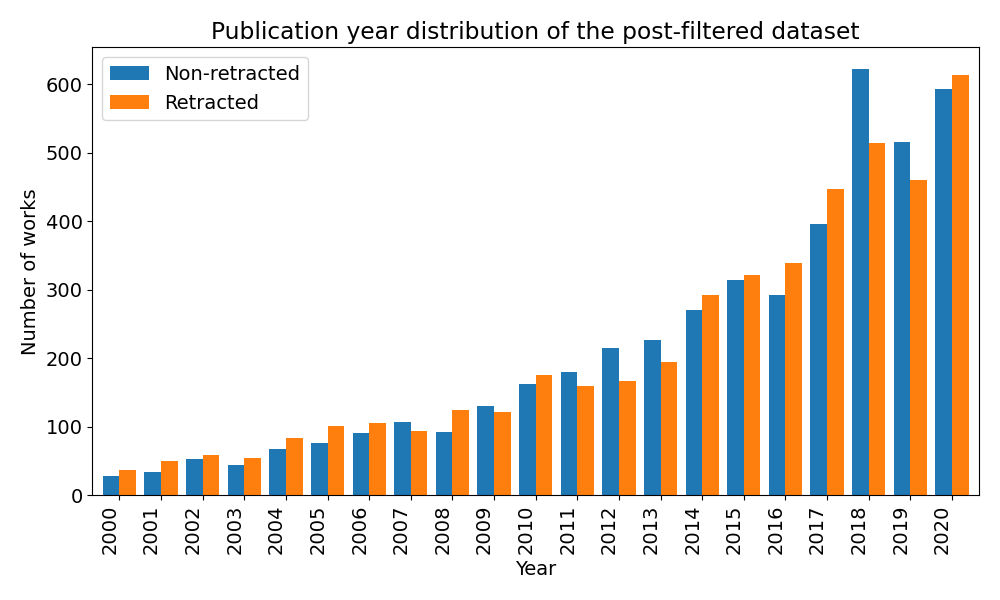
\includegraphics[width=1\linewidth]{output.png}
    \caption{Publication year distribution for retracted and non-retracted works.}
    \label{fig:publication_parity}
\end{figure}



% \begin{figure}[h]
%     \centering
%     \includegraphics[width=0.75\linewidth]{images/NormalisedRetractionGraph.png}
%     \caption{Comparison of our dataset and Retraction Watch Dataset when normalised between 0 and 1}
%     \label{fig:normalised_comparision}
% \end{figure}

In the generated dataset, 7.54\% of the articles reported as retracted in Retraction Watch were not marked as retracted by OpenAlex, possibly because OpenAlex's metadata is derived from multiple input sources. This discrepancy further illustrates the difficulty of identifying retracted research since it may not be labelled as such. This discrepancy has been recently directly addressed with CrossRef integrating the Retraction Watch database into the metadata returned from their API~\cite{rittman_retraction_2025}.

% The disparity between articles flagged as retracted between both datasets was not explored, as the process used by both databases to update information has many factors (such Retraction Watches open source nature, or OpenAlex's metadata being derived from multiple input sources).


Analysis of correlations between journal features revealed two notable findings:
\begin{enumerate}
    \item A weak, significant positive correlation between the work count log and the retraction count log (Pearson correlation coefficient 0.065, p-value \(<\) 0.05). This seems counterintuitive, as more retractions are likely to occur given more publications, and hence, a strong positive correlation would be present. This finding could indicate that journals that publish fewer works are less proactive at detecting potential retractions or that publishing research that will be retracted is more complicated within journals with greater work output, presumably due to increased scrutiny of these works. 
    
    \item A strong negative correlation between the retraction count and log of h-index (Pearson correlation coefficient -0.656, p-value \(<\) 0.05). This relationship is expected. The h-index, a widely used measure of a journal's productivity and impact, is based on its most cited papers. Typically when a work is considered for inclusion in a journal or conference, a peer reviewer is tasked with subjecting that research to the scrutiny of others who are experts in the same field \cite{banks_thoughts_2018}. This reviewer is sourced from academics who review for many reasons (primarily altruistic), such as keeping up with the latest developments, building associations with journals, and demonstrating a commitment to the scientific field \cite{steer_peer_2021}. Importantly, time available to review is a finite resource \cite{warne_rewarding_2016}. It is likely that more reviewers are available for greater h-index journals. Publishing venues with higher h-index values potentially have a more rigorous peer review process, authors are more diligent when submitting to these journals, or higher-quality journals attract better-quality research.

\end{enumerate}

\subsection{Classifier Performance}

Results for all classifiers are presented in Table \ref{tab:classifier-scores-new}, showing performance for both the retracted and not retracted classes. The highest-scoring approaches for each metric are highlighted in bold. Commercial models were excluded from further analysis as all commercial models responded that no research was retracted within the testing dataset. This was thought to be due to the safety restrictions implemented within these models, which prevented responses that could be considered problematic \cite{bai2022constitutionalaiharmlessnessai}. 


All models outperformed random guessing (i.e. 0.5 as this is a binary classification task), although the improvement varies considerably between models. The highest accuracy (0.682) is achieved by \gls*{llama} 3.2-base, although accuracy scores overall are generally higher for more traditional feature-based approaches such as gradient boost, \gls*{svm}, \gls*{xgb}, and Random Forest achieved superior precision compared to the more modern contextually aware \glspl*{llm}.
% The table also reveals that Llama 3.2-base achieved the highest precision (0.682), recall (0.682) and F1 score (0.682).

Regarding the retracted class, \gls*{svm} achieved the highest precision (0.690) and \gls*{llama} 3.2-base the highest recall (0.683). Interestingly, both instruction-tuned decoder-based \glspl*{llm} (Gemma 2-instruct and \gls*{llama} 3.2-instruct) also achieve high recall for the retracted class but this is achieved by predicting retracted for the majority of instances, as demonstrated by the very low recall for the non-retracted class. This could be due to instruction tuning, as they are trained to be more cautious and risk-averse, indicating that instruction-tuned models might not be suitable for this type of classification task. 

\begin{table}[htbp]
\caption{Retraction classifier performance results.}\label{tab:classifier-scores-new}
\small
\begin{tabular}{l*{7}{c}}
\toprule
\multirow{2}{*}{Model} & \multirow{2}{*}{Acc.} & \multicolumn{3}{c}{Non-Retracted} & \multicolumn{3}{c}{Retracted} \\
\cmidrule(lr){3-5} \cmidrule(lr){6-8}
& & P & R & F1 & P & R & F1 \\
\midrule
Logistic Regression & 0.638 & 0.638 & 0.647 & 0.642 & 0.639 & 0.630 & 0.635 \\
Decision Tree & 0.568 & 0.570 & 0.574 & 0.572 & 0.568 & 0.564 & 0.566 \\
Random Forest & 0.666 & 0.648 &\textbf {0.731} & \textbf{0.687} & 0.689 & 0.601 & 0.642 \\
\gls*{svm} & 0.671 & 0.655 & 0.725 & 0.688 & \textbf{0.690} & 0.616 & 0.651 \\
\gls*{xgb} & 0.665 & 0.654 & 0.705 & 0.679 & 0.678 & 0.624 & 0.650 \\
AdaBoost & 0.631 & 0.619 & 0.684 & 0.650 & 0.645 & 0.577 & 0.609 \\
Super Learner & 0.669 & 0.661 & 0.699 & 0.680 & 0.678 & 0.640 & 0.659 \\
\gls*{mlp} & 0.655 & 0.650 & 0.675 & 0.663 & 0.660 & 0.634 & 0.647 \\
Gemma 2-base & 0.553 & 0.615 & 0.292 & 0.396 & 0.534 & 0.816 & 0.645 \\
Gemma 2-instruct & 0.529 &\textbf{ 0.730} & 0.098 & 0.173 & 0.515 & \textbf{0.963} & 0.671 \\
\gls*{bert} & 0.609 & 0.612 & 0.602 & 0.607 & 0.606 & 0.616 & 0.611\\
BioBERT & 0.608 & 0.598 & 0.668 & 0.631  & 0.621 & 0.548  & 0.582\\
\gls*{llama} 3.2-base & \textbf{0.682} &0.686 & 0.674 & 0.680  & 0.678 &  0.689  & \textbf{0.683}\\
\gls*{llama} 3.2-instruct & 0.535 & 0.714 & 0.121 & 0.208  & 0.518 &  0.951  & 0.671\\
\bottomrule
\end{tabular}
\end{table}






These findings establish baseline results using the dataset. 
%% However, these finding needs to be contextualised within the objectives of this investigation itself. The study aimed to establish baseline results for the generated data set rather than to optimise individual model performance. 
%In particular, BERT, as a pre-trained model, typically requires extensive fine-tuning on large, domain-specific datasets to leverage its capabilities, which was not the case here. The limited fine-tuning described in the study (up to 10 epochs in the training data) may have been insufficient to achieve superior precision performance in this domain.

% Furthermore, BERT was limited to 512 tokens, which could have truncated important information for this model, given the verbosity of the abstracts. The feature-based classifiers did not have this limitation. Furthermore, while BERT and BioBERT's precision was lower than traditional machine learning models, it demonstrated comparative performance in other metrics, such as recall and the F1 score. This finding could suggest that different model approaches could excel in different evaluation metrics.

%Importantly, investigations into appropriate model selection lay the groundwork for future investigations. Optimising the performance of these approaches, particularly for specific metrics such as precision, remains an open challenge for this data set.




%% \input{Chapters/investigations/ablation_studies}
\subsection{Ablation Analysis}

The importance of individual features to the feature-based classification models was explored by conducting an ablation study on all input features. Datasets were created for each feature by permuting the data to exclude that feature and then averaging the evaluation metrics (F1 score, precision, recall, accuracy) across all models for each ablation. Lower scoring metrics indicate a greater contribution to the performance of a classifier.
% \begin{table}[H]
% \caption{Average Ablation Model Scores: lowest scoring ablations are in bold.\label{tab7}}
% \begin{tabularx}{\textwidth}{rrrrr}
% \toprule
% Ablation & Accuracy & Precision & Recall & f1 Score \\\midrule
% Abstract & 0.655 & 0.657 & 0.655 & 0.654 \\
% Citation Count & 0.648 & 0.649 & 0.647 & 0.647 \\
% First Author & 0.649 & 0.651 & 0.649 & 0.648 \\
% First Author Countries & 0.649 & 0.650 & 0.649 & 0.648 \\
% Primary Topic & 0.644 & 0.646 & 0.644 & 0.643 \\
% Publication Year & \textbf{0.641} & \textbf{0.643} & \textbf{0.641} & \textbf{0.640} \\
% Title & 0.648 & 0.649 & 0.648 & 0.647 \\
% \bottomrule
%     \label{tab:ablation_scores}
% \end{tabularx}
% \end{table}

\begin{table}[htbp]
\caption{Ablation performance metrics: lowest scoring ablations are in bold.}\label{tab:ablation}
\small
\begin{tabular}{l*{7}{c}}
\toprule
\multirow{2}{*}{Model} & \multirow{1}{*}{Acc.}  & \multicolumn{3}{c}{Non-Retracted} & \multicolumn{3}{c}{Retracted} \\
\cmidrule(lr){3-5} \cmidrule(lr){6-8}
 & & P & R & F1 & P & R & F1 \\
\midrule
Abstract & 0.655 & 0.670 & 0.612 & 0.638 & 0.645 & 0.678 & 0.669 \\
Citation Count & 0.648 & 0.659 & 0.611 & 0.634 & 0.638 & 0.684 & 0.660 \\
First Author & 0.649 & 0.662 & 0.609 & 0.634 & 0.639 & 0.689 & 0.663 \\
First Author Countries & 0.649 & 0.663 & 0.604 & 0.632 & 0.638 & 0.693 & 0.664 \\
Primary Topic & 0.644 & 0.658 & 0.602 & 0.628 & 0.634 & 0.687 & 0.659 \\
Publication Year & \textbf{0.641} & \textbf{0.656} & \textbf{0.594} & \textbf{0.622} & \textbf{0.630} & \textbf{0.688} & \textbf{0.657} \\
Title & 0.648 & 0.657 & 0.618 & 0.636 & 0.641 & 0.678 & 0.658 \\
\bottomrule
\end{tabular}
\end{table}
% \begin{table}[H] 
% \caption{Average Ablation Model Scores: lowest scoring ablation are in bold.\label{tab7}}
% \begin{tabularx}{\textwidth}{rrrrr}
% \toprule
% Ablation  &  Accuracy &  Precision &  Recall &  f1 Score \\
% % Ablation                &           &            &         &           \\
% \midrule
% Abstract Inverted Index &     \textbf{0.629} &      0.648 &   \textbf{0.556} &     \textbf{0.597} \\
% Citation Count        &     0.635 &      0.654 &   0.565 &     0.605 \\
% First Author            &     0.633 &      0.648 &   0.574 &     0.607 \\
% First Author Countries  &     0.632 &      \textbf{0.644} &   0.590 &     0.613 \\
% Primary Topic           &     0.633 &      0.651 &   0.560 &     0.601 \\
% Publication Date        &     0.630 &      0.645 &   0.570 &     0.604 \\
% Title                   &     0.638 &      0.652 &   0.582 &     0.613 \\
% \bottomrule
%     \label{tab:ablation_scores}
% \end{tabularx}
% \end{table}

% Averaged ablation study results are reported in Table \ref{tab:ablation_scores}. 
% % and visualised in Figure \ref{fig:average_ablation}. 
% Interestingly, within the ablation studies, the average lowest-scoring precision ablation (0.644) was achieved by ablating First Author Countries. For all other metrics, the lowest average scored metric was achieved by ablating the Abstract (Accuracy 0.629, Recall 0.556, F1 Score 0.597). 

% \begin{figure}
%     \centering
%     \includegraphics[width=1\linewidth]{images/classifier_results.png}
%     \caption{Different evaluation metrics on the test dataset.}
%     \label{fig:classifer-scores}
% \end{figure}

% \begin{figure}
%     \centering
%     \includegraphics[width=1\linewidth]{images/ablation_average_score.png}
%     \caption{Average model scores per ablation study.}
%     \label{fig:average_ablation}
% \end{figure}


% \begin{table}[H] 

% \begin{tabularx}{\textwidth}{Xrrrr}

% \toprule
%         {} & F Value  & Num DF & Deb DF &  Pr \text{>} F\\
%         \toprule
%     Metric     &  220.4789 & 3.0000 & 18.00000 & 0.0000 \\
%     \end{tabularx}

%     \caption{Repeated Measures ANOVA for evaluation metric and ablations}
%     \label{tab:anova}
% \end{table}

% A repeated measures ANOVA demonstrates that there are significant differences among the evaluation metrics across all ablations, indicating the choice of evaluation metrics significant impacts ablation importance - see Table \ref{tab:anova}.

Several observations on the ablation of features can be made given the results reported in Table \ref{tab:ablation}.
% and Figure \ref{fig:average_ablation}.
The publication year proved to be the most crucial feature, with its ablation resulting in the lowest scores across all metrics. This suggests that temporal information plays a more significant role in classification than detailed textual content, which is logical given the increase in publications and the corresponding increase in retractions. This temporal information component also highlights the challenge that traditional classification approaches potentially face in this area; given that publication year is such a strong signal, its presence might eclipse other valuable contributions from other features. The Primary Topic feature also demonstrated substantial importance, producing the second-lowest scores when ablated. Reduction in performance when First Author Countries are ablated provides some indication of the likelihood that a work will be retracted, supporting previous findings \cite{stretton_publication_2012}.

Contrary to what might be intuitively expected, the abstract, despite being the longest and most detailed textual component, emerged as the least influential feature across all evaluation metrics. When ablated, it yielded the highest average scores for accuracy (0.655), precision (0.657), recall (0.655), and F1 score (0.654), indicating its removal had the least negative impact on model performance. This counterintuitive finding regarding the abstract's limited influence could be attributed to several factors. First, structured metadata features (like publication date and primary topic) may provide more consistent and unambiguous signals for classification compared to the potentially noisy and variable nature of abstract text. Second, there might be considerable information redundancy between the abstract and other textual features like the title, making its individual contribution less distinctive. 
% outlined in the introduction.


\section{Discussion}\label{sec:Discussion}



% \subsection{Journal Metadata analysis}

% Two notable findings were reported from the analysis of the journal metadata: a weak significant positive correlation between a journal's log of work found and the log of retraction count and a strong negative correlation between the journals' retraction count and log of a journal H index. This seems counterintuitive, as more retractions are likely to occur given more publications, and hence, a strong positive correlation would be present. This interesting finding could indicate that journals that publish fewer works are less proactive at detecting potential retractions or that publishing research that will be retracted is more complicated within journals with greater work output, presumably due to increased scrutiny of these works. The strong negative correlation between the retraction count and the log of the h-index indicates that as a journal's h-index increases, its retraction count tends to decrease significantly, which is expected. 

% The h-index, a widely used measure of a journal's productivity and impact, is based on its most cited papers. Typically when a work is considered for inclusion in a journal or conference, a peer reviewer is tasked with subjecting that research to the scrutiny of others who are experts in the same field \cite{banks_thoughts_2018}. This reviewer is sourced from academics who review for many, primarily, altruistic reasons, such as keeping up with the latest developments, building associations with journals, and demonstrating a commitment to the scientific field \cite{steer_peer_2021}. Importantly, not every researcher is a peer reviewer, which means that available review time is a finite resource \cite{warne_rewarding_2016}. It is likely that more reviwers are available for greater h-index journals. Publishing venues with higher h-index values potentially have a more rigorous peer review process, authors are more diligent when submitting to these journals, or higher-quality journals attract better-quality research.



% Understanding the scope of this problem requires understanding what safeguards are in place. When research is considered for inclusion in a journal or conference, a peer reviewer is tasked with subjecting that research to the scrutiny of others who are experts in the same field \cite{banks_thoughts_2018}. The reviewer then makes a biased judgement about whether a paper should be accepted for publication in a journal. Reviewers themselves review for many, primarily altruistic reasons, such as keeping up with the latest developments, building associations with journals, and demonstrating a commitment to the scientific field \cite{steer_peer_2021}. Importantly, not every researcher is a peer reviewer, which means that available review time is a finite resource \cite{warne_rewarding_2016}. Given the increased publication rate and retractions observed within the literature, efficient allocation of the reviewer resource would allow reviewers to spend more time analysing good-quality research.

% \subsection{Machine Learning For Predicting Retractions}
% This research demonstrates that machine learning techniques are appropriate for exploring and predicting article retractions. In particular, more traditional feature-based approaches such as gradient boost, SVM, XGBoost, and Random Forest achieved superior precision compared to the more modern contextually aware BERT model. However, this finding needs to be contextualised within the objectives of this investigation itself. The study aimed to establish baseline results for the generated data set rather than to optimise individual model performance. In particular, BERT, as a pre-trained model, typically requires extensive fine-tuning on large, domain-specific datasets to leverage its capabilities, which was not the case here. The limited fine-tuning described in the study (5 epochs on the training data) may have needed to have been sufficient to achieve superior precision performance in this domain.
% Furthermore, BERT was limited to 512 tokens, which could have truncated important information for this model, given the verbosity of the abstracts. The feature-based classifiers did not have this limitation. Furthermore, while BERT's precision was lower than traditional machine learning models, it demonstrated comparative performance in other metrics, such as recall and the F1 score. This finding could suggest that different model approaches could excel in different evaluation metrics.

% Importantly, investigations into appropriate model selection lay the groundwork for future investigations. Optimising the performance of these approaches, particularly for specific metrics such as precision, remains an open challenge for this data set. Future work could explore more extensive fine-tuning of BERT and more elaborate feature engineering within feature-based classifier models.


% \subsection{Ablations}

% Several observations on the ablation of features can be made given the results reported in Table \ref{tab:ablation_scores} and Figure \ref{fig:average_ablation}. Unsurprisingly, given the amount of information contained within an abstract, it appears to be the most influential feature among all feature-based models when considering recall or F1 score, as when ablated, it resulted in the lowest average scores for accuracy (0.629), recall (0.556) and F1 score (0.597). This suggests that the abstract contains significant information to identify potentially retracted articles. Interestingly, ablating the "First Author Countries" feature resulted in the lowest precision score (0.644). This indicates that the geographical origin of the first author provides valuable information for precise classification, which supports previous work outlined in the introduction.

% \subsection {Coefficient Analysis}

% Certain coefficients (words) were associated with the data set classes (retraction / non-retraction). Although analysis of this is speculative, the author suggests the reasons why certain coefficients were associated with classes as follows:

% \begin{enumerate}
%     \item ``Randomized" was strongly associated with a paper retraction; this could be due to the increased scrutiny that this type of research is subjected to (such as medical/health domains).
%     \item ``Contrary", which is likely to be seen in papers contradictory to established ideas, is less likely to have been retracted.
%     \item ``Indirectly" and "Benefits" have negative coefficients, which could suggest that more cautious or nuanced claims are less likely to be retracted.
%     \item The presence of particular names (``Mohammad" and ``Gao") could indicate some geographic or cultural factors in retractions, supporting previous research in this area \cite{stretton_publication_2012}.
% \end{enumerate}

% \subsection{Application within Peer Review}
Machine learning approaches can successfully identify retracted papers using a created open-access dataset. 


One of the potential applications of the classifier described above is as a tool during the peer review process, in much the same way that text similarity tools are often used to identify potential plagiarism. The required level of precision or recall would depend on how the tools would be used. If used as a screening tool to flag potentially problematic papers for additional review, a high recall would be preferable to avoid missing articles that are subsequently retracted. However, if used as a check which a submitted article must pass then high precision would be necessary to avoid the suppression of valid research. The performance of the models reported above, while promising, indicates that identification of retracted articles is not a trivial prediction task and may not be sufficient for some purposes. The decision regarding the involvement of systems to detect potential retractions within the peer review process is ultimately the choice of publishers. 

% \subsection{Ethics of Automating Retraction Prediction}
The automatic prediction of potential retractions also raises ethical concerns. Predictive models, such as the ones described here, can introduce bias thereby raising potential fairness issues \cite{caton2024fairness,mehrabi2021survey}.  
% Although these approaches offer promising tools for improving research integrity, they also present significant challenges that current methodologies have not adequately addressed. These concerns also partially explain why precision was the evaluation metric focused on when interpreting the results. 
% A primary concern is that these models are correlations rather than causal. For instance, the coefficient analysis revealed an association between retraction likelihood and the presence of certain features, such as use of cautious language (e.g., ``indirectly," ``benefits") and particular names. 
% This limitation may inadvertently perpetuate existing biases within the publication system. 
% For instance, the coefficient analysis revealed an association between cautious language (e.g., ``indirectly," ``benefits") and retraction likelihood. 
% The models presented within this work are correlational and not causal, meaning bias can be inadvertently output. 
Such biases can unfairly penalise the groups more likely to be identified as producing research that will be retracted (e.g., first authors from particular locations) while benefiting those it is less likely to identify. This could introduce inductive bias into investigations, potentially leading to unforeseen consequences in the scientific publishing landscape, such as influencing which research questions are investigated and which methodologies are applied. In addition, authors may attempt to report results in ways that avoid detection by these models, potentially leading to self-censorship or overly cautious reporting of results. Conversely, bad actors with knowledge of these models may exploit that information to avoid detection, potentially facilitating the dissemination of invalid results. 

An important consideration is how best to apply these models in practice. While machine learning classifiers can highlight publications at higher risk of retraction, final decisions on whether a paper should be investigated or retracted must rest with human experts—editors, reviewers, and domain specialists. For example, automated models flag potential anomalies in medical and clinical contexts, but the ultimate judgment requires expert oversight \cite{prictor_where_2023, funer_responsibility_2023}. Similarly, the classifiers reported here are intended to aid decision-making rather than stand-alone arbiters of scientific validity. A fully automated retraction process is not desirable, nor is it necessarily the duty of model developers to initiate or recommend retraction investigations on every flagged paper. Instead, these outputs can be a starting point for further human-led scrutiny. This workflow ensures that any potential reasons for retraction—which may be multifaceted and not always captured by the model—are carefully examined. It also prevents the undue penalisation of authors, institutions, or countries that might otherwise be overrepresented due to biases in the training data. By maintaining a robust human-in-the-loop process, publishers and editorial boards can leverage model predictions ethically and effectively to uphold the reliability of the scientific record.



\section{Limitations}

This study has several notable limitations. The study design relied on a single data source, the Retraction Watch database, which provides valuable but incomplete coverage. The presence of ``stealth retractions'', wherein papers are removed without official notice or may not be reported to Retraction Watch, creates the potential for missed or under-detected retractions. Additionally, it was retrospective, using data from 2000 to 2020, which limits the ability to assess the models' real-time or prospective effectiveness in detecting erroneous work at publication. Theoretical limitations exist within the model choice, as they capture correlational rather than causal relationships, potentially leading to false positives or negatives, as using these patterns can misrepresent the underlying reasons for retractions. Data was sampled from 2000 to 2020, which would not represent more recent changes in retracted works. Since 2020, there have been innovative natural language generation models that could potentially increase the count of retracted works. Features that are not fully representative of a piece of research were used. Due to copyright restrictions, abstracts and metadata were used rather than full-text articles. Indicators of methodological errors or unsupported conclusions might appear in the main text and not the title and abstract, potentially reducing the reliability of our retraction-prediction metrics.

Additionally, some \gls*{llm} may have been partly trained on the same corpus used to develop or validate our dataset, inflating their performance scores. This issue does not affect purely feature-based approaches but undermines the reliability of \gls*{llm}-derived results. Features such as the first author’s country or institution may reflect systemic biases in scientific publishing rather than genuine predictors of flawed work. Such biases risk penalising authors from certain regions or affiliations if used in editorial decision-making. Models may overfit to spurious textual or demographic correlations in the training data, leading to unjustified flags or missed detections when applied to new, diverse datasets.

% These limitations highlight the need for further research using broader data sources, more comprehensive (full-text) analyses, prospective validation, and systematic bias checks to ensure fair and accurate retraction predictions.


\section{Conclusions}
\label{sec:Conclusions}

This research demonstrates the potential of machine learning approaches in predicting retracted articles, contributing to efforts aimed at enhancing the integrity of scientific publication. By creating a novel open-source dataset that combines information from the Retraction Watch database and the OpenAlex API, a resource for future investigations in this area has been contributed. Our dataset encompasses 9,028  articles published between 2000 and 2020, evenly divided between retracted and non-retracted works, and includes a variety of features such as abstracts, citation metrics, and author information.

Experiments showed that, with the exception of the recently released \gls*{llama} 3.2 base model, traditional feature-based classifiers, such as gradient boosting machines and \glspl*{svm}, outperformed contextual language models like \gls*{bert}, BioBERT, and Gemma in terms of precision. The best-performing model achieved a precision of 0.690, indicating that while machine learning techniques hold promise, there remains a need for significant improvement before they can be effectively integrated into the peer review process. The ablation study highlighted the importance of the publication year, primary topic and the first author's country in predicting retractions, aligning with previous findings that suggest certain demographics may be more prone to retractions due to various factors.

%% We also addressed the ethical considerations of automating retraction predictions. The potential for biases, especially relating to geographic and cultural factors, underscores the need for careful interpretation and responsible application of these models. It is crucial to ensure that such tools do not inadvertently discriminate against researchers or stifle innovative work that challenges established paradigms.

\subsection{Future work}

There is potential for the approaches described here to be extended by making use of additional information with the potential to assist in the identification of retracted research. For example, the citation network of references to a paper and the references within the paper itself may provide useful information. In addition, the models described here analysed abstracts, but analysis of the full text itself could potentially allow models to evaluate flaws in methodology, result synthesis or false conclusions. Finally, analysis of the full author list of an article could reveal patterns of collaboration or even help to identify potential paper mills. 

% Another avenue for future research is investigation of domain impact on retraction. This is an important area to explore, as retraction rates and reasons may vary significantly across different scientific disciplines, such as biomedical, physics or social sciences. Analysing these domain-specific trends could lead to more tailored and effective retraction prediction models.

%% Our current models utilise abstracts and metadata, which, in effect, is an abstraction of the full text. Analysis of the full text itself could potentially allow models to evaluate flaws in methodology, result synthesis or false conclusions. Furthermore, this approach uses first authors as a feature while research typically has multiple authors attached to them, which, when assessed together, could reveal patterns of collaboration or even potential paper mills.

% Moved from earlier
% We have focused on established features which have been demonstrated to impact the likelihood of retraction. The ablation study revealed that the abstract content and the first author's country were particularly important features. However, this is not to say there aren't more features which might provide better results. For example, citation networks of references to a paper are likely to reflect the quality of the work, or indeed the references within the paper itself potentially being an indicator of potential retraction.


\section{List of Abbreviations}

\printglossary[type=\acronymtype]

\section*{Declarations}
\subsection*{Ethics approval and consent to participate}

Not applicable.

\subsection*{Consent for publication}

Not applicable.

\subsection*{Availability of data and material}
\label{sec:Data Availability}
The dataset supporting the conclusions of this article is available in the Predicting Article Retractions repository \cite{noauthor_anonymized_nodate}.

\subsection*{Competing interests}
The authors declare that they have no competing interests.


\subsection*{Funding}
\label{sec:Funding}
This work was supported by the Centre for Doctoral Training in Speech and Language Technologies (SLT) and their Applications funded by UK Research and Innovation [grant number EP/S023062/1].


\subsection*{Authors' contributions }

AF contributed to this research's conception, design analysis, data interpretation, and submission drafting. MS contributed to this research's conception, design analysis, data interpretation, and submission drafting. All authors read and approved the final manuscript.


\subsection*{Open Access}
For the purpose of open access, the authors have applied a Creative Commons Attribution (CC BY) licence to any Author Accepted Manuscript version arising.


 % \footnote{https://anonymous.4open.science/r/RetractionWatch/}.



% \section{Results}\label{sec2}

% Sample body text. Sample body text. Sample body text. Sample body text. Sample body text. Sample body text. Sample body text. Sample body text.

% \section{This is an example for first level head---section head}\label{sec3}

% \subsection{This is an example for second level head---subsection head}\label{subsec2}

% \subsubsection{This is an example for third level head---subsubsection head}\label{subsubsec2}

% Sample body text. Sample body text. Sample body text. Sample body text. Sample body text. Sample body text. Sample body text. Sample body text. 

% \section{Equations}\label{sec4}

% Equations in \LaTeX\ can either be inline or on-a-line by itself (``display equations''). For
% inline equations use the \verb+$...$+ commands. E.g.: The equation
% $H\psi = E \psi$ is written via the command \verb+$H \psi = E \psi$+.

% For display equations (with auto generated equation numbers)
% one can use the equation or align environments:
% \begin{equation}
% \|\tilde{X}(k)\|^2 \leq\frac{\sum\limits_{i=1}^{p}\left\|\tilde{Y}_i(k)\right\|^2+\sum\limits_{j=1}^{q}\left\|\tilde{Z}_j(k)\right\|^2 }{p+q}.\label{eq1}
% \end{equation}
% where,
% \begin{align}
% D_\mu &=  \partial_\mu - ig \frac{\lambda^a}{2} A^a_\mu \nonumber \\
% F^a_{\mu\nu} &= \partial_\mu A^a_\nu - \partial_\nu A^a_\mu + g f^{abc} A^b_\mu A^a_\nu \label{eq2}
% \end{align}
% Notice the use of \verb+\nonumber+ in the align environment at the end
% of each line, except the last, so as not to produce equation numbers on
% lines where no equation numbers are required. The \verb+\label{}+ command
% should only be used at the last line of an align environment where
% \verb+\nonumber+ is not used.
% \begin{equation}
% Y_\infty = \left( \frac{m}{\textrm{GeV}} \right)^{-3}
%     \left[ 1 + \frac{3 \ln(m/\textrm{GeV})}{15}
%     + \frac{\ln(c_2/5)}{15} \right]
% \end{equation}
% The class file also supports the use of \verb+\mathbb{}+, \verb+\mathscr{}+ and
% \verb+\mathcal{}+ commands. As such \verb+\mathbb{R}+, \verb+\mathscr{R}+
% and \verb+\mathcal{R}+ produces $\mathbb{R}$, $\mathscr{R}$ and $\mathcal{R}$
% respectively (refer Subsubsection~\ref{subsubsec2}).

% \section{Tables}\label{sec5}

% Tables can be inserted via the normal table and tabular environment. To put
% footnotes inside tables you should use \verb+\footnotetext[]{...}+ tag.
% The footnote appears just below the table itself (refer Tables~\ref{tab1} and \ref{tab2}). 
% For the corresponding footnotemark use \verb+\footnotemark[...]+

% \begin{table}[h]
% \caption{Caption text}\label{tab1}%
% \begin{tabular}{@{}llll@{}}
% \toprule
% Column 1 & Column 2  & Column 3 & Column 4\\
% \midrule
% row 1    & data 1   & data 2  & data 3  \\
% row 2    & data 4   & data 5\footnotemark[1]  & data 6  \\
% row 3    & data 7   & data 8  & data 9\footnotemark[2]  \\
% \botrule
% \end{tabular}
% \footnotetext{Source: This is an example of table footnote. This is an example of table footnote.}
% \footnotetext[1]{Example for a first table footnote. This is an example of table footnote.}
% \footnotetext[2]{Example for a second table footnote. This is an example of table footnote.}
% \end{table}

% \noindent
% The input format for the above table is as follows:

% %%=============================================%%
% %% For presentation purpose, we have included  %%
% %% \bigskip command. Please ignore this.       %%
% %%=============================================%%
% \bigskip
% \begin{verbatim}
% \begin{table}[<placement-specifier>]
% \caption{<table-caption>}\label{<table-label>}%
% \begin{tabular}{@{}llll@{}}
% \toprule
% Column 1 & Column 2 & Column 3 & Column 4\\
% \midrule
% row 1 & data 1 & data 2	 & data 3 \\
% row 2 & data 4 & data 5\footnotemark[1] & data 6 \\
% row 3 & data 7 & data 8	 & data 9\footnotemark[2]\\
% \botrule
% \end{tabular}
% \footnotetext{Source: This is an example of table footnote. 
% This is an example of table footnote.}
% \footnotetext[1]{Example for a first table footnote.
% This is an example of table footnote.}
% \footnotetext[2]{Example for a second table footnote. 
% This is an example of table footnote.}
% \end{table}
% \end{verbatim}
% \bigskip
% %%=============================================%%
% %% For presentation purpose, we have included  %%
% %% \bigskip command. Please ignore this.       %%
% %%=============================================%%

% \begin{table}[h]
% \caption{Example of a lengthy table which is set to full textwidth}\label{tab2}
% \begin{tabular*}{\textwidth}{@{\extracolsep\fill}lcccccc}
% \toprule%
% & \multicolumn{3}{@{}c@{}}{Element 1\footnotemark[1]} & \multicolumn{3}{@{}c@{}}{Element 2\footnotemark[2]} \\\cmidrule{2-4}\cmidrule{5-7}%
% Project & Energy & $\sigma_{calc}$ & $\sigma_{expt}$ & Energy & $\sigma_{calc}$ & $\sigma_{expt}$ \\
% \midrule
% Element 3  & 990 A & 1168 & $1547\pm12$ & 780 A & 1166 & $1239\pm100$\\
% Element 4  & 500 A & 961  & $922\pm10$  & 900 A & 1268 & $1092\pm40$\\
% \botrule
% \end{tabular*}
% \footnotetext{Note: This is an example of table footnote. This is an example of table footnote this is an example of table footnote this is an example of~table footnote this is an example of table footnote.}
% \footnotetext[1]{Example for a first table footnote.}
% \footnotetext[2]{Example for a second table footnote.}
% \end{table}

% In case of double column layout, tables which do not fit in single column width should be set to full text width. For this, you need to use \verb+\begin{table*}+ \verb+...+ \verb+\end{table*}+ instead of \verb+\begin{table}+ \verb+...+ \verb+\end{table}+ environment. Lengthy tables which do not fit in textwidth should be set as rotated table. For this, you need to use \verb+\begin{sidewaystable}+ \verb+...+ \verb+\end{sidewaystable}+ instead of \verb+\begin{table*}+ \verb+...+ \verb+\end{table*}+ environment. This environment puts tables rotated to single column width. For tables rotated to double column width, use \verb+\begin{sidewaystable*}+ \verb+...+ \verb+\end{sidewaystable*}+.

% \begin{sidewaystable}
% \caption{Tables which are too long to fit, should be written using the ``sidewaystable'' environment as shown here}\label{tab3}
% \begin{tabular*}{\textheight}{@{\extracolsep\fill}lcccccc}
% \toprule%
% & \multicolumn{3}{@{}c@{}}{Element 1\footnotemark[1]}& \multicolumn{3}{@{}c@{}}{Element\footnotemark[2]} \\\cmidrule{2-4}\cmidrule{5-7}%
% Projectile & Energy	& $\sigma_{calc}$ & $\sigma_{expt}$ & Energy & $\sigma_{calc}$ & $\sigma_{expt}$ \\
% \midrule
% Element 3 & 990 A & 1168 & $1547\pm12$ & 780 A & 1166 & $1239\pm100$ \\
% Element 4 & 500 A & 961  & $922\pm10$  & 900 A & 1268 & $1092\pm40$ \\
% Element 5 & 990 A & 1168 & $1547\pm12$ & 780 A & 1166 & $1239\pm100$ \\
% Element 6 & 500 A & 961  & $922\pm10$  & 900 A & 1268 & $1092\pm40$ \\
% \botrule
% \end{tabular*}
% \footnotetext{Note: This is an example of table footnote this is an example of table footnote this is an example of table footnote this is an example of~table footnote this is an example of table footnote.}
% \footnotetext[1]{This is an example of table footnote.}
% \end{sidewaystable}

% \section{Figures}\label{sec6}

% As per the \LaTeX\ standards you need to use eps images for \LaTeX\ compilation and \verb+pdf/jpg/png+ images for \verb+PDFLaTeX+ compilation. This is one of the major difference between \LaTeX\ and \verb+PDFLaTeX+. Each image should be from a single input .eps/vector image file. Avoid using subfigures. The command for inserting images for \LaTeX\ and \verb+PDFLaTeX+ can be generalized. The package used to insert images in \verb+LaTeX/PDFLaTeX+ is the graphicx package. Figures can be inserted via the normal figure environment as shown in the below example:

% %%=============================================%%
% %% For presentation purpose, we have included  %%
% %% \bigskip command. Please ignore this.       %%
% %%=============================================%%
% \bigskip
% \begin{verbatim}
% \begin{figure}[<placement-specifier>]
% \centering
% \includegraphics{<eps-file>}
% \caption{<figure-caption>}\label{<figure-label>}
% \end{figure}
% \end{verbatim}
% \bigskip
% %%=============================================%%
% %% For presentation purpose, we have included  %%
% %% \bigskip command. Please ignore this.       %%
% %%=============================================%%

% \begin{figure}[h]
% \centering
% \includegraphics[width=0.9\textwidth]{fig.eps}
% \caption{This is a widefig. This is an example of long caption this is an example of long caption  this is an example of long caption this is an example of long caption}\label{fig1}
% \end{figure}

% In case of double column layout, the above format puts figure captions/images to single column width. To get spanned images, we need to provide \verb+\begin{figure*}+ \verb+...+ \verb+\end{figure*}+.

% For sample purpose, we have included the width of images in the optional argument of \verb+\includegraphics+ tag. Please ignore this. 

% \section{Algorithms, Program codes and Listings}\label{sec7}

% Packages \verb+algorithm+, \verb+algorithmicx+ and \verb+algpseudocode+ are used for setting algorithms in \LaTeX\ using the format:

% %%=============================================%%
% %% For presentation purpose, we have included  %%
% %% \bigskip command. Please ignore this.       %%
% %%=============================================%%
% \bigskip
% \begin{verbatim}
% \begin{algorithm}
% \caption{<alg-caption>}\label{<alg-label>}
% \begin{algorithmic}[1]
% . . .
% \end{algorithmic}
% \end{algorithm}
% \end{verbatim}
% \bigskip
% %%=============================================%%
% %% For presentation purpose, we have included  %%
% %% \bigskip command. Please ignore this.       %%
% %%=============================================%%

% You may refer above listed package documentations for more details before setting \verb+algorithm+ environment. For program codes, the ``verbatim'' package is required and the command to be used is \verb+\begin{verbatim}+ \verb+...+ \verb+\end{verbatim}+. 

% Similarly, for \verb+listings+, use the \verb+listings+ package. \verb+\begin{lstlisting}+ \verb+...+ \verb+\end{lstlisting}+ is used to set environments similar to \verb+verbatim+ environment. Refer to the \verb+lstlisting+ package documentation for more details.

% A fast exponentiation procedure:

% \lstset{texcl=true,basicstyle=\small\sf,commentstyle=\small\rm,mathescape=true,escapeinside={(*}{*)}}
% \begin{lstlisting}
% begin
%   for $i:=1$ to $10$ step $1$ do
%       expt($2,i$);  
%       newline() od                (*\textrm{Comments will be set flush to the right margin}*)
% where
% proc expt($x,n$) $\equiv$
%   $z:=1$;
%   do if $n=0$ then exit fi;
%      do if odd($n$) then exit fi;                 
%         comment: (*\textrm{This is a comment statement;}*)
%         $n:=n/2$; $x:=x*x$ od;
%      { $n>0$ };
%      $n:=n-1$; $z:=z*x$ od;
%   print($z$). 
% end
% \end{lstlisting}

% \begin{algorithm}
% \caption{Calculate $y = x^n$}\label{algo1}
% \begin{algorithmic}[1]
% \Require $n \geq 0 \vee x \neq 0$
% \Ensure $y = x^n$ 
% \State $y \Leftarrow 1$
% \If{$n < 0$}\label{algln2}
%         \State $X \Leftarrow 1 / x$
%         \State $N \Leftarrow -n$
% \Else
%         \State $X \Leftarrow x$
%         \State $N \Leftarrow n$
% \EndIf
% \While{$N \neq 0$}
%         \If{$N$ is even}
%             \State $X \Leftarrow X \times X$
%             \State $N \Leftarrow N / 2$
%         \Else[$N$ is odd]
%             \State $y \Leftarrow y \times X$
%             \State $N \Leftarrow N - 1$
%         \EndIf
% \EndWhile
% \end{algorithmic}
% \end{algorithm}

% %%=============================================%%
% %% For presentation purpose, we have included  %%
% %% \bigskip command. Please ignore this.       %%
% %%=============================================%%
% \bigskip
% \begin{minipage}{\hsize}%
% \lstset{frame=single,framexleftmargin=-1pt,framexrightmargin=-17pt,framesep=12pt,linewidth=0.98\textwidth,language=pascal}% Set your language (you can change the language for each code-block optionally)
% %%% Start your code-block
% \begin{lstlisting}
% for i:=maxint to 0 do
% begin
% { do nothing }
% end;
% Write('Case insensitive ');
% Write('Pascal keywords.');
% \end{lstlisting}
% \end{minipage}

% \section{Cross referencing}\label{sec8}

% Environments such as figure, table, equation and align can have a label
% declared via the \verb+\label{#label}+ command. For figures and table
% environments use the \verb+\label{}+ command inside or just
% below the \verb+\caption{}+ command. You can then use the
% \verb+\ref{#label}+ command to cross-reference them. As an example, consider
% the label declared for Figure~\ref{fig1} which is
% \verb+\label{fig1}+. To cross-reference it, use the command 
% \verb+Figure \ref{fig1}+, for which it comes up as
% ``Figure~\ref{fig1}''. 

% To reference line numbers in an algorithm, consider the label declared for the line number 2 of Algorithm~\ref{algo1} is \verb+\label{algln2}+. To cross-reference it, use the command \verb+\ref{algln2}+ for which it comes up as line~\ref{algln2} of Algorithm~\ref{algo1}.

% \subsection{Details on reference citations}\label{subsec7}

% Standard \LaTeX\ permits only numerical citations. To support both numerical and author-year citations this template uses \verb+natbib+ \LaTeX\ package. For style guidance please refer to the template user manual.

% Here is an example for \verb+\cite{...}+: \cite{bib1}. Another example for \verb+\citep{...}+: \citep{bib2}. For author-year citation mode, \verb+\cite{...}+ prints Jones et al. (1990) and \verb+\citep{...}+ prints (Jones et al., 1990).

% All cited bib entries are printed at the end of this article: \cite{bib3}, \cite{bib4}, \cite{bib5}, \cite{bib6}, \cite{bib7}, \cite{bib8}, \cite{bib9}, \cite{bib10}, \cite{bib11}, \cite{bib12} and \cite{bib13}.


% \section{Examples for theorem like environments}\label{sec10}

% For theorem like environments, we require \verb+amsthm+ package. There are three types of predefined theorem styles exists---\verb+thmstyleone+, \verb+thmstyletwo+ and \verb+thmstylethree+ 

% %%=============================================%%
% %% For presentation purpose, we have included  %%
% %% \bigskip command. Please ignore this.       %%
% %%=============================================%%
% \bigskip
% \begin{tabular}{|l|p{19pc}|}
% \hline
% \verb+thmstyleone+ & Numbered, theorem head in bold font and theorem text in italic style \\\hline
% \verb+thmstyletwo+ & Numbered, theorem head in roman font and theorem text in italic style \\\hline
% \verb+thmstylethree+ & Numbered, theorem head in bold font and theorem text in roman style \\\hline
% \end{tabular}
% \bigskip
% %%=============================================%%
% %% For presentation purpose, we have included  %%
% %% \bigskip command. Please ignore this.       %%
% %%=============================================%%

% For mathematics journals, theorem styles can be included as shown in the following examples:

% \begin{theorem}[Theorem subhead]\label{thm1}
% Example theorem text. Example theorem text. Example theorem text. Example theorem text. Example theorem text. 
% Example theorem text. Example theorem text. Example theorem text. Example theorem text. Example theorem text. 
% Example theorem text. 
% \end{theorem}

% Sample body text. Sample body text. Sample body text. Sample body text. Sample body text. Sample body text. Sample body text. Sample body text.

% \begin{proposition}
% Example proposition text. Example proposition text. Example proposition text. Example proposition text. Example proposition text. 
% Example proposition text. Example proposition text. Example proposition text. Example proposition text. Example proposition text. 
% \end{proposition}

% Sample body text. Sample body text. Sample body text. Sample body text. Sample body text. Sample body text. Sample body text. Sample body text.

% \begin{example}
% Phasellus adipiscing semper elit. Proin fermentum massa
% ac quam. Sed diam turpis, molestie vitae, placerat a, molestie nec, leo. Maecenas lacinia. Nam ipsum ligula, eleifend
% at, accumsan nec, suscipit a, ipsum. Morbi blandit ligula feugiat magna. Nunc eleifend consequat lorem. 
% \end{example}

% Sample body text. Sample body text. Sample body text. Sample body text. Sample body text. Sample body text. Sample body text. Sample body text.

% \begin{remark}
% Phasellus adipiscing semper elit. Proin fermentum massa
% ac quam. Sed diam turpis, molestie vitae, placerat a, molestie nec, leo. Maecenas lacinia. Nam ipsum ligula, eleifend
% at, accumsan nec, suscipit a, ipsum. Morbi blandit ligula feugiat magna. Nunc eleifend consequat lorem. 
% \end{remark}

% Sample body text. Sample body text. Sample body text. Sample body text. Sample body text. Sample body text. Sample body text. Sample body text.

% \begin{definition}[Definition sub head]
% Example definition text. Example definition text. Example definition text. Example definition text. Example definition text. Example definition text. Example definition text. Example definition text. 
% \end{definition}

% Additionally a predefined ``proof'' environment is available: \verb+\begin{proof}+ \verb+...+ \verb+\end{proof}+. This prints a ``Proof'' head in italic font style and the ``body text'' in roman font style with an open square at the end of each proof environment. 

% \begin{proof}
% Example for proof text. Example for proof text. Example for proof text. Example for proof text. Example for proof text. Example for proof text. Example for proof text. Example for proof text. Example for proof text. Example for proof text. 
% \end{proof}

% Sample body text. Sample body text. Sample body text. Sample body text. Sample body text. Sample body text. Sample body text. Sample body text.

% \begin{proof}[Proof of Theorem~{\upshape\ref{thm1}}]
% Example for proof text. Example for proof text. Example for proof text. Example for proof text. Example for proof text. Example for proof text. Example for proof text. Example for proof text. Example for proof text. Example for proof text. 
% \end{proof}

% \noindent
% For a quote environment, use \verb+\begin{quote}...\end{quote}+
% \begin{quote}
% Quoted text example. Aliquam porttitor quam a lacus. Praesent vel arcu ut tortor cursus volutpat. In vitae pede quis diam bibendum placerat. Fusce elementum
% convallis neque. Sed dolor orci, scelerisque ac, dapibus nec, ultricies ut, mi. Duis nec dui quis leo sagittis commodo.
% \end{quote}

% Sample body text. Sample body text. Sample body text. Sample body text. Sample body text (refer Figure~\ref{fig1}). Sample body text. Sample body text. Sample body text (refer Table~\ref{tab3}). 

% \section{Methods}\label{sec11}

% Topical subheadings are allowed. Authors must ensure that their Methods section includes adequate experimental and characterization data necessary for others in the field to reproduce their work. Authors are encouraged to include RIIDs where appropriate. 

% \textbf{Ethical approval declarations} (only required where applicable) Any article reporting experiment/s carried out on (i)~live vertebrate (or higher invertebrates), (ii)~humans or (iii)~human samples must include an unambiguous statement within the methods section that meets the following requirements: 

% \begin{enumerate}[1.]
% \item Approval: a statement which confirms that all experimental protocols were approved by a named institutional and/or licensing committee. Please identify the approving body in the methods section

% \item Accordance: a statement explicitly saying that the methods were carried out in accordance with the relevant guidelines and regulations

% \item Informed consent (for experiments involving humans or human tissue samples): include a statement confirming that informed consent was obtained from all participants and/or their legal guardian/s
% \end{enumerate}

% If your manuscript includes potentially identifying patient/participant information, or if it describes human transplantation research, or if it reports results of a clinical trial then  additional information will be required. Please visit (\url{https://www.nature.com/nature-research/editorial-policies}) for Nature Portfolio journals, (\url{https://www.springer.com/gp/authors-editors/journal-author/journal-author-helpdesk/publishing-ethics/14214}) for Springer Nature journals, or (\url{https://www.biomedcentral.com/getpublished/editorial-policies\#ethics+and+consent}) for BMC.

% \section{Discussion}\label{sec12}

% Discussions should be brief and focused. In some disciplines use of Discussion or `Conclusion' is interchangeable. It is not mandatory to use both. Some journals prefer a section `Results and Discussion' followed by a section `Conclusion'. Please refer to Journal-level guidance for any specific requirements. 

% \section{Conclusion}\label{sec13}

% Conclusions may be used to restate your hypothesis or research question, restate your major findings, explain the relevance and the added value of your work, highlight any limitations of your study, describe future directions for research and recommendations. 

% In some disciplines use of Discussion or 'Conclusion' is interchangeable. It is not mandatory to use both. Please refer to Journal-level guidance for any specific requirements. 

% \backmatter

% \bmhead{Supplementary information}

% If your article has accompanying supplementary file/s please state so here. 

% Authors reporting data from electrophoretic gels and blots should supply the full unprocessed scans for key as part of their Supplementary information. This may be requested by the editorial team/s if it is missing.

% Please refer to Journal-level guidance for any specific requirements.

% \bmhead{Acknowledgements}

% Acknowledgements are not compulsory. Where included they should be brief. Grant or contribution numbers may be acknowledged.

% Please refer to Journal-level guidance for any specific requirements.

% \section*{Declarations}

% Some journals require declarations to be submitted in a standardised format. Please check the Instructions for Authors of the journal to which you are submitting to see if you need to complete this section. If yes, your manuscript must contain the following sections under the heading `Declarations':

% \begin{itemize}
% \item Funding
% \item Conflict of interest/Competing interests (check journal-specific guidelines for which heading to use)
% \item Ethics approval and consent to participate
% \item Consent for publication
% \item Data availability 
% \item Materials availability
% \item Code availability 
% \item Author contribution
% \end{itemize}

% \noindent
% If any of the sections are not relevant to your manuscript, please include the heading and write `Not applicable' for that section. 

% %%===================================================%%
% %% For presentation purpose, we have included        %%
% %% \bigskip command. Please ignore this.             %%
% %%===================================================%%
% \bigskip
% \begin{flushleft}%
% Editorial Policies for:

% \bigskip\noindent
% Springer journals and proceedings: \url{https://www.springer.com/gp/editorial-policies}

% \bigskip\noindent
% Nature Portfolio journals: \url{https://www.nature.com/nature-research/editorial-policies}

% \bigskip\noindent
% \textit{Scientific Reports}: \url{https://www.nature.com/srep/journal-policies/editorial-policies}

% \bigskip\noindent
% BMC journals: \url{https://www.biomedcentral.com/getpublished/editorial-policies}
% \end{flushleft}

% \begin{appendices}

% \section{Section title of first appendix}\label{secA1}

% An appendix contains supplementary information that is not an essential part of the text itself but which may be helpful in providing a more comprehensive understanding of the research problem or it is information that is too cumbersome to be included in the body of the paper.

% %%=============================================%%
% %% For submissions to Nature Portfolio Journals %%
% %% please use the heading ``Extended Data''.   %%
% %%=============================================%%

% %%=============================================================%%
% %% Sample for another appendix section			       %%
% %%=============================================================%%

% %% \section{Example of another appendix section}\label{secA2}%
% %% Appendices may be used for helpful, supporting or essential material that would otherwise 
% %% clutter, break up or be distracting to the text. Appendices can consist of sections, figures, 
% %% tables and equations etc.

% \end{appendices}

%%===========================================================================================%%
%% If you are submitting to one of the Nature Portfolio journals, using the eJP submission   %%
%% system, please include the references within the manuscript file itself. You may do this  %%
%% by copying the reference list from your .bbl file, paste it into the main manuscript .tex %%
%% file, and delete the associated \verb+\bibliography+ commands.                            %%
%%===========================================================================================%%

\bibliography{sn-bibliography}% common bib file
%% if required, the content of .bbl file can be included here once bbl is generated
%%\input sn-article.bbl


\end{document}
